\documentclass[a4paper]{article}

\usepackage[utf8]{inputenc}
\usepackage[OT1]{fontenc}

\usepackage[vmargin = 10ex, hmargin = 6em]{geometry}

\usepackage{graphicx}

\usepackage{array}

\renewcommand{\arraystretch}{1.2}
\setlength{\tabcolsep}{4pt}
\setlength{\leftmargini}{1em}
\setlength{\leftmarginii}{1.5em}

\begin{document}

\thispagestyle{empty}

\fbox{%
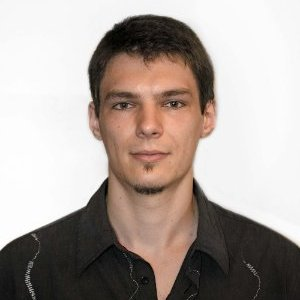
\includegraphics[height=10ex]{./gb.jpg}
\hspace{1em}
\begin{minipage}[t]{.3\textwidth}
	\setlength{\tabcolsep}{2pt}
	\begin{tabular}{r l}
		\multicolumn{2}{c}{\Large Guillaume Bono} \\
		\hline
		{\small born on:} &
			November 22nd, 1992 \\
		{\small in:} &
			Bron, (69) France
	\end{tabular}
\end{minipage}
}
\hfill
\begin{minipage}[t]{.5\textwidth}
	\flushright
	\setlength{\tabcolsep}{2pt}
	\begin{tabular}{r l}
		
\includegraphics[height=2ex]{./home.png} : &
			22 rue Thénard \\
		 &
			69008, Lyon (France) \\

		
\includegraphics[height=2ex]{./phone.png} : &
			+33 6 85 07 97 05 \\
		
\includegraphics[height=2ex]{./mail.png} : &
			guillaume.bono@inria.fr
	\end{tabular}
\end{minipage}

\vfill

\centering
\fbox{%
	\Large Curriculum Vitae
}

\vfill

\centering
\begin{tabular}{>{\small}r c >{\small}l l r r}
	
\includegraphics[height=3ex]{./edu.png} &
		\multicolumn{5}{l}{Education} \\
	\hline
	Oct. 2016 &- &today      &PhD Student in AI                      &INSA Lyon, INRIA         &(69, France) \\
		&\multicolumn{5}{l}{$\rightarrow$ {\footnotesize Member of INRIA team Chroma at CITI Laboratory of INSA Lyon, with support of Volvo Group}} \\
		&\multicolumn{5}{l}{$\bullet$ {\footnotesize Subject: Multi-Agent Deep Reinforcement Learning for Dynamic and Stochastis Vehicle Routing Problems}} \\
		&\multicolumn{5}{l}{$\bullet$ {\footnotesize Supervisors: Jilles Dibangoye, La\"etitia Matignon, Florian Pereyron, Olivier Simonin}} \\
		&\multicolumn{5}{l}{$\bullet$ {\footnotesize Pub. : [JFPDA-2017]} {\scriptsize ``Problèmes dynamiques et stochastiques de collectes et de livraisons par véhicules intelligents''}} \\
		&\multicolumn{5}{l}{$\bullet$ {\footnotesize Pub. : [JFPDA-2018]} {\scriptsize ``Sur le Gradient de la Politique pour les Systèmes Multi-Agents Coopératifs''}} \\
		&\multicolumn{5}{l}{$\bullet$ {\footnotesize Pub. : [ECML-2018]} {\scriptsize ``Cooperative Multi-Agent Policy Gradient''}} \\
		&\multicolumn{5}{l}{$\bullet$ {\footnotesize Pub. : [PGMRL-2018]} {\scriptsize ``Simulation of Stochastic Vehicle Routing Problems in Urban Environment'' }} \\
		&\multicolumn{5}{l}{$\bullet$ {\footnotesize Pub. : [T-ITS-2020]} {\scriptsize ``Solving Multi-Agent Routing Problems using Deep Attention Mechanisms''}} \\
		&\multicolumn{5}{l}{$\Rightarrow$ {\footnotesize 1\textsuperscript{st} Summer School on Cognitive Robotics by MERS group at MIT CSAIL}} \\
		&\multicolumn{5}{l}{$\Rightarrow$ {\footnotesize Institut d'Automne en Intelligence Artificielle (Summer School on AI) by GDRIA (french AI Research Group)}} \\
	Aug. 2014 &- &May 2016   &Master of Computer Science (GPA: 3.89) &GeorgiaTech              &(GA, USA) \\
		&\multicolumn{5}{l}{$\rightarrow$ {\footnotesize Computational Perception and Robotics: adv. algorithms, ML, autonomous robotics, CV, …}} \\
		&\multicolumn{5}{l}{$\bullet$ {\footnotesize Project: Autonomous navigation with WiFi mapping, energy management, obstacle avoidance}} \\
		&\multicolumn{5}{l}{$\bullet$ {\footnotesize Project: Face detection and masks warping with GUI}} \\
	Sep. 2012 &- &Feb. 2016  &Engineering Degree (GPA: 4.0)          &Supélec                  &(91, France) \\
		&\multicolumn{5}{l}{$\rightarrow$ {\footnotesize Interactive Systems and Robotics: programming, electronics, control, signal/image proc. , ML, …}} \\
		&\multicolumn{5}{l}{$\bullet$ {\footnotesize Project: Remote controlled lake plateform with algal bloom monitoring and status report to distant server}} \\
		&\multicolumn{5}{l}{$\bullet$ {\footnotesize Project: Integrated PWM circuit design on professional software \emph{Cadence Virtuoso}}} \\
	Sep. 2010 &- &June 2012  &Prepartory Classes                     &La Martinière Monplaisir &(69, France) \\
		&\multicolumn{5}{l}{$\rightarrow$ {\footnotesize Maths, Physics and Engineering}} \\
	Sep. 2006 &- &June 2010  &High School diploma                    &La Martinière Monplaisir &(69, France) \\
	\\
	
\includegraphics[height=3ex]{./work.png} &
		\multicolumn{5}{l}{Professional Experience} \\
	\hline
	Apr. 2015 &- &Dec. 2015  &Internship \& Research Engineer &Awabot                   &(69, France)\\
		&\multicolumn{5}{l}{$\bullet$ {\footnotesize Gestures recognition for home companion robot implementing DNN with \emph{Caffe} on \emph{nVidia Tegra K1}}} \\
	\\
	
\includegraphics[height=3ex]{./perso.png} &
		\multicolumn{5}{l}{Personal Experience}\\
	\hline
	Sep. 2012 &- &June 2014  &Sound systems Tech. Manager     &Sono Supélec             &(91, France)\\
		&\multicolumn{5}{l}{$\rightarrow$ {\footnotesize Concert organization, events animation, logistics, technical troubleshooting, sound engineer}} \\
\end{tabular}

\vfill

\begin{minipage}[t]{.3\textwidth}
	\underline{
		
\includegraphics[height=3ex]{./lang.png}
		Languages:
	}
	\begin{itemize}
		\item[] 
\includegraphics[height=1.5ex]{./fr-flag.png} French (native)
		\item[] 
\includegraphics[height=1.5ex]{./uk-flag.png} English (B2-C1)
			\begin{itemize}
				\item TOEFL iBT 105/120
				\item GRE
			\end{itemize}
		\item[] \includegraphics[height=1.5ex]{./ger-flag.png} German (B1-B2)
		\item[] 
\includegraphics[height=1.5ex]{./cn-flag.png} Chinese (A1)
	\end{itemize}
\end{minipage}
\hfill
\begin{minipage}[t]{.3\textwidth}
	\underline{
		
\includegraphics[height=3ex]{./comp.png}
		Computer Skills:
	}
	\begin{itemize}
		\item Programming Languages:
			\begin{itemize}
				\item C, C++, Python, Java
			\end{itemize}
		\item Libraries:
			\begin{itemize}
				\item STL, Boost, OpenCV
				\item Caffe, Scikit-learn, Pytorch
				\item Android ...
			\end{itemize}
		\item CUDA, ROS
		\item Git, Subversion
		\item LaTeX, Microsoft Office Suite
	\end{itemize}
\end{minipage}
\hfill
\begin{minipage}[t]{.3\textwidth}
	\underline{
		
\includegraphics[height=3ex]{./games.png}
		Hobbies:
	}
	\begin{itemize}
		\item Computer:
			\begin{itemize}
				\item Video-games, e-Sport
				\item Hardware, Robots
			\end{itemize}
		\item Music:
			\begin{itemize}
				\item Guitar
				\item Sound systems, Mixing
			\end{itemize}
		\item Board-games, RPG
		\item Books and Films:
			\begin{itemize}
				\item Fantasy, SF
			\end{itemize}
	\end{itemize}
\end{minipage}

\end{document}
